\documentclass{article}

\usepackage{graphicx}
\usepackage{txfonts}
\usepackage{subfigure}
\usepackage{epstopdf}
\usepackage{lineno}
\usepackage[authoryear,round]{natbib}
\usepackage[backref]{hyperref}
\usepackage{url}
\usepackage[inline]{enumitem}
\usepackage{verbatim}
\usepackage{csquotes}
\bibliographystyle{swsc.bst}

\begin{document}
\title{Manuscript Ref: swsc160029}
\maketitle
\section*{Response}

\begin{enumerate}
\item \emph{Comparison with existing Dst models}

\textbf{Remarks}: 

The authors would like to bring to attention figures \ref{fig:rmseNew} and \ref{fig:ccNew} in which we test the performance NARMAX (\emph{NM}) model as specified in \cite{balikhin:narmax} on the 63 storms benchmark set of \cite{Ji2012}, but use previously predicted $Dst$ values as suggested by the referee instead of actual $Dst$ data. %Beginning from the year $1998$ we generate predictions for the \emph{NM} model till the year $2006$. 
This is denoted by \emph{NM Variant} in the figures. As observed in figures \ref{fig:rmseNew} and \ref{fig:ccNew} this leads to severe degradation of performance. 

This leads us to conclude that the following statement from \cite{Ji2012} applies only to the testing of the \emph{TL} model: \blockquote{When run the Dst model program for calculating the prediction value of Dst, we do not use the observed Dst data. We use the only previously predicted Dst data.}

Furthermore, the authors do not agree that comparisons should be made only on models that input the same input parameters. For practical reasons, one may be interested in comparing models’ predictions, irrespective of the input parameters. Space weather users care only about the accuracy of the model’s prediction and should not care what parameters the model inputs.


\begin{figure}
   \centering
   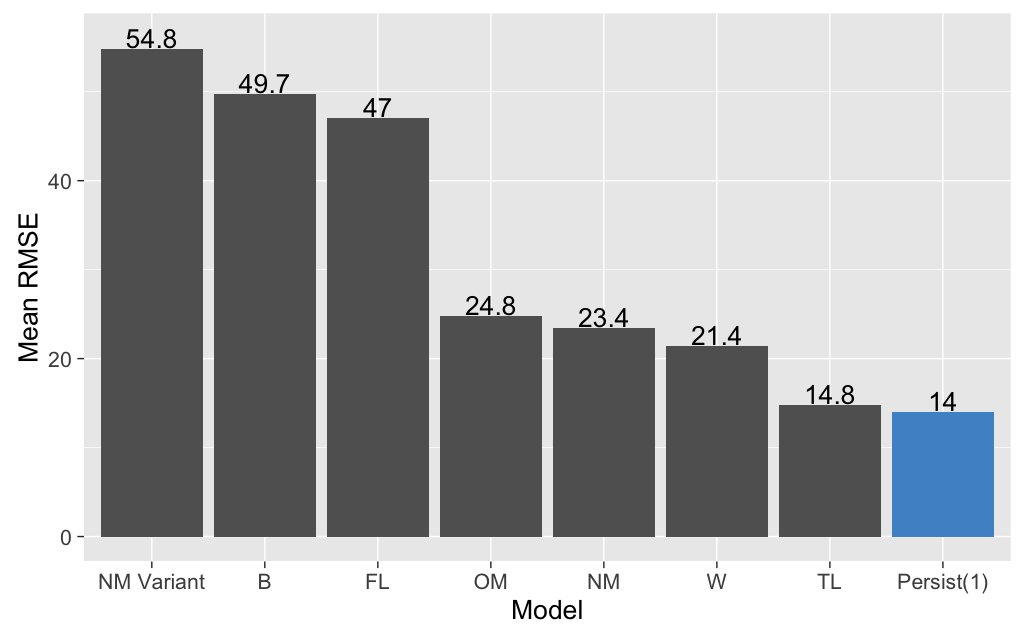
\includegraphics[width=\textwidth]{Compare_RMSE_New.png}
      \caption{
      Averaged RMSE performance of \emph{NARMAX Variant} and the 
      \emph{Persistence} model versus results in \cite{Ji2012}.
      }
      \label{fig:rmseNew}
\end{figure}

\begin{figure}
   \centering
   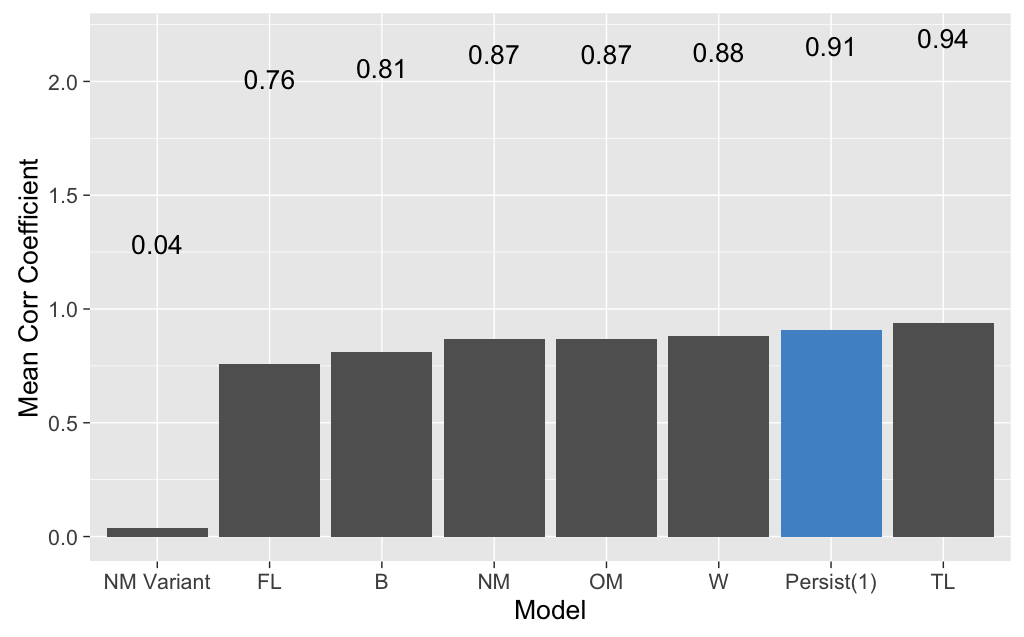
\includegraphics[width=\textwidth]{Compare_CC_New.png}
      \caption{Averaged cross correlation performance of \emph{NARMAX Variant} and the 
      \emph{Persistence} model versus results in \citet{Ji2012}.}
         \label{fig:ccNew}
\end{figure}

\item \emph{Differences between quicklook, provisional and final $Dst$}

\textbf{Remarks}: If the differences among final, quicklook, and provisional $Dst$ are the quite days base line values (as the reviewer suggests), then this would not affect the timing of the storms only the magnitude due to the subtraction of different offsets. Also, this would not change the evaluation of delta $Dst$, CC, RMSE, etc., provided that we consistently use the same type of Dst (e.g, we use only provisional or quicklook $Dst$s).
 


\end{enumerate}

\section*{Acknowledgements}

The authors would like to thank the reviewer for dedicating their time to provide constructive and valuable feedback. 

\bibliography{swsc}


\end{document}